% Chapter 10

\chapter{Background Estimation} % Chapter title
\label{ch:backgrounds} 

This analysis requires two leptons that reconstruct to a $Z$ mass, jets, \met, and \HT. Any standard model processes that produce this signature will appear as a background to the search. The most important task of the analysis is to identify and estimate these backgrounds, so that any excess of events appearing on top of the standard model background can be identified. The main backgrounds for this analysis are described in \autoref{ch:background_processes}. The largest background is from flavor symmetric processes, with smaller contributions coming from diboson processes, \dyjets, rare top processes, and fake and non-prompt leptons.

%----------------------------------------------------------------------------------------

\section{Flavor Symmetric Processes}
\label{sec:bg-fs}

\ac{FS} backgrounds include any processes that produce pairs of leptons with uncorrelated flavor in the final state. In this analysis, the largest contribution comes from \ttbar, with additional events from processes like $WW$ and $Z\rightarrow\tau\tau$. In these processes, each lepton comes from a different decay. Unlike a $Z\rightarrow\ll$ decay then, these leptons' flavors are completely independent. 

\subsection{Flavor Symmetry Method}
\label{sec:method-fs}
As a consequence of the independence of the lepton flavors, any \ac{FS} process should produce $ee$, $\mu\mu$, and $e\mu$ events in a 1:1:2 ratio. This ratio is taken advantage of by the flavor symmetry method by measuring $e\mu$ events in data and using them to predict the contribution of these processes in the $ee$ and $\mu\mu$ channels. 

To estimate the number of events in SRZ, a control region called CR-FS is used. Both regions are defined in \autoref{tab:regions-z}. CR-FS is very similar to SRZ with two changes: it requires different-flavor leptons instead of the same-flavor leptons required by SRZ, and the \mll range it covers has been expanded by a factor of three, now ranging from 61 to 121 \gev. The expansion of the \mll window is done to increase the number of events in the control region, thus lowering the statistical uncertainty of the prediction\footnote{Though this statistical uncertainty is no longer dominant for the analysis, the method was developed for a smaller dataset for which this expansion dramatically decreased the total uncertainty on the background prediction. \cite{zmet} Because of previous excesses seen, the signal region was not reoptimized for the larger dataset used in this search, but in future iterations of this analysis, the signal region have tighter cuts, making this decreased statistical uncertainty significant once again.}. 

This control region is expected to be about 95\% pure in \ac{FS} processes, with most of the remaining events coming from fake or non-prompt leptons. The \ac{FS} portion is made up primarily of \ttbar ($\sim$80\%), with additional contributions from $Wt$ ($\sim$10\%), $WW$ ($\sim$10\%), and $<1$\% $Z \rightarrow \tau\tau$. 

After the number of data events are measured in CR-FS, correction factors are applied to account for trigger efficiencies, selection efficiencies, the \mll expansion, and the purity of the control region. Combining these factors, the estimate for number of events in the $ee$ and $\mu\mu$ channels is as follows:

\begin{eqnarray}
N_{ee}^\text{est} = \frac{1}{2} \cdot  f_{\mathrm{FS}} \cdot f_{Z \mathrm{\text{-}mass}} \cdot\sum^{N_{e\mu}^\text{data}} k_{e}(\pT^{\mu}, \eta^{\mu})\cdot \alpha(\pT^{\ell_1}, \eta^{\ell_1}) ,\\
N_{\mu\mu}^\text{est} = \frac{1}{2} \cdot  f_{\mathrm{FS}} \cdot f_{Z \mathrm{\text{-}mass}} \cdot \sum^{N_{e\mu}^\text{data}}k_{\mu}(\pT^{e}, \eta^{e})\cdot \alpha(\pT^{\ell_1}, \eta^{\ell_1}) ,
\end{eqnarray}

\noindent where $N_{e\mu}^\text{data}$ is the number of data events observed in CR-FS, 
$k_{e}(\pT, \eta)$ and $k_{\mu}(\pT, \eta)$ are relative selection efficiencies for electrons and muons, calculated in bins of $\pT$ and $\eta$ of the lepton to be replaced, 
and $\alpha(\pT, \eta)$ accounts for the different trigger efficiencies for events in each channel, binned based on the kinematics of the leading lepton. These $k$ and $\alpha$ factors are calculated in an inclusive on-$Z$ selection ($81<\mll/\GeV<101$, $\geq2$ jets), 
according to:

\begin{eqnarray}\label{eq:kfac}
k_{e}(\pT, \eta) = \sqrt{\frac{N_{ee}^{\text{meas}}}{N_{\mu\mu}^{\text{meas}}}} \\
k_{\mu}(\pT, \eta) = \sqrt{\frac{N_{\mu\mu}^{\text{meas}}}{N_{ee}^{\text{meas}}}} \\
\alpha(\pT, \eta) = \frac{\sqrt{\epsilon^\text{trig}_{ee}(\pt,\eta)\times\epsilon^\text{trig}_{\mu\mu}(\pt,\eta)}}{\epsilon^\text{trig}_{e\mu}(\pt,\eta)}
\label{eq:kandalpha}
\end{eqnarray}

\noindent where $\epsilon^\text{trig}_{ee/\mu\mu}$ is the trigger efficiency 
\footnote{This efficiency is defined by taking all events in the inclusive on-$Z$ selection mentioned above and determining the fraction that passes the relevant trigger requirement defined by \autoref{tab:trigger_strat}. Because the offline selection made on these events already has some trigger dependence, this calculation of efficiency could be slightly biased. This effect is considered in \autoref{sec:unc_fs}, and the uncertainty applied to the estimate as a result is described.} 
and $N_{ee/\mu\mu}^{\text{meas}}$ 
is the number of $ee/\mu\mu$ events in the inclusive on-$Z$ region described above. 
Here $k_{e}(\pT, \eta)$ = $1/k_{\mu}(\pT, \eta)$, and this $k$ factor is calculated separately for leading and sub-leading leptons, and the appropriate $k$ value is selected based on the position of the lepton to be replaced. 

Electron, muon, and trigger efficiencies are all quite close to one, and as a consequence, these correction factors are typically within 10\% of unity, except in the region $|\eta|<0.1$ where, because of the lack of coverage of the muon spectrometer, they are up to 50\% from unity.

The estimate is corrected for contamination of non-\ac{FS} backgrounds in CR-FS. A scaling factor is determined by subtracting these backgrounds from the number of $e\mu$ events measured in CR-FS, then determining the fraction of the original data events that this pure-\ac{FS} number represents. The estimate for the other backgrounds is taken from \ac{MC} for all processes except fakes, which are predicted from data using the matrix method described in \autoref{sec:bg-fake}. 

A prediction is made both for the signal region, SRZ, and the lower-\met validation region, VRS. This process is performed separately for the two data taking periods, 2015 and 2016, because of the changing triggers and conditions. The results are then summed together, as shown in \autoref{tab:fs_yields}. The uncertainties in this table are discussed in \autoref{sec:unc_fs}.

\begin{table}
\begin{center}
 \begin{tabular}{lccc}
   \hline 
   Region & $ee$ prediction & $\mu\mu$ prediction & combined prediction \\
   \hline
   \hline
   \multicolumn{4}{c}{Prediction for 14.7~\ifb\ of 2015+2016 Data} \\
   \hline
SRZ & $ 16.50 \pm 2.11 $ & $ 16.67 \pm 2.04 $ & $ 33.16 \pm 3.94 $ \\
VRS & $ 49.70 \pm 4.61 $ & $ 49.60 \pm 4.56 $ & $ 99.31 \pm 8.47 $ \\
\hline
\hline
 \end{tabular}
\end{center}
 \caption{
   Yields in signal and validation regions for the flavor symmetric background. 
Errors include statistical uncertainty, uncertainty from MC closure, uncertainty from the k and $\alpha$ factors, 
uncertainty due to deriving triggers efficiencies from a DAOD, and uncertainty on the MC shape used to correct for the \mll expansion. 
 }
 \label{tab:fs_yields}
\end{table}

\subsection{Sideband Fit Method}
\label{sec:method-sideband}

As a crosscheck to the flavor symmetry method, a \ac{MC}-based method is used. This method is called a ``sideband fit,'' and it begins with a \ac{MC} estimate of the signal region across a \mll range that includes all values above 40 \gev. This region, excluding the on-$Z$ range that makes up the \ac{SR}, is used as a control region, defined as CRT in \autoref{tab:regions-z}. 

The total data yield is measured in CRT, and the \ac{MC} is fit to match this yield with one normalization factor which scales the overall \ttbar background. As mentioned in the previous section, \ttbar is the dominant \ac{FS} background, making up about 80\% of the total events. All other backgrounds contributing to this control region are constrained by their uncertainties, which are used as nuisance parameters in the fit. The normalization factor from this fit is then applied to the \ttbar \ac{MC} yield in the \ac{SR}, and combined with the \ac{MC} predictions of the other \ac{FS} processes in the \ac{SR} to give a final estimate of this background. The results of the fit can be seen in \autoref{tab:Yields_sideband_mc}. 



\begin{sidewaystable*}
\begin{center}
\setlength{\tabcolsep}{0.0pc}
{\small
%%
\begin{tabular*}{\textwidth}{@{\extracolsep{\fill}}lrrrr}
\noalign{\smallskip}\hline\noalign{\smallskip}
{\bf  channel}           & $ee/\mu\mu$ CRT            & $ee/\mu\mu$ SRZ            & $ee$ SRZ            & $\mu\mu$ SRZ              \\[-0.05cm]
\noalign{\smallskip}\hline\noalign{\smallskip}
%%
Observed events          & $273$              & $60$              & $35$              & $25$                    \\
\noalign{\smallskip}\hline\noalign{\smallskip}
%%
Fitted bkg events         & $272.8 \pm 16.9$          & $49.3 \pm 8.0$          & $27.1 \pm 4.7$          & $22.7 \pm 3.8$              \\
\noalign{\smallskip}\hline\noalign{\smallskip}
%%
        Fitted flavour symmetry events         & $237.0 \pm 21.7$          & $29.0 \pm 7.5$          & $16.4 \pm 4.3$          & $12.6 \pm 3.3$              \\
%%
        Fitted $WZ/ZZ$ events         & $4.0 \pm 1.1$          & $14.3 \pm 4.5$          & $7.8 \pm 2.5$          & $6.5 \pm 2.1$              \\
%%
        Fitted {\sc Sherpa} \dyjets\ events         & $2.0 \pm 0.1$          & --          & --          & --              \\
%%
        Data-driven \dyjets (\gjets) events         & --          & $3.1 \pm 2.3$          & $1.0_{-1.0}^{+1.3}$          & $2.1 \pm 1.4$              \\
%%
        Fitted rare top events         & $4.0 \pm 1.0$          & $2.9 \pm 0.8$          & $1.4 \pm 0.4$          & $1.5 \pm 0.4$              \\
%%
        Data-driven fake lepton events         & $25.8 \pm 14.3$          & $0.10_{-0.10}^{+0.18}$          & $0.46 \pm 0.45$          & $0.10 \pm 0.01$              \\
%%     
 \noalign{\smallskip}\hline\noalign{\smallskip}
%%
Expected \ac{SM} Events              & $366.7$          & $61.0$          & $33.7$          & $27.7$              \\
\noalign{\smallskip}\hline\noalign{\smallskip}
%%
        MC flavour symmetry events         & $331.3$          & $40.7$          & $23.1$          & $17.6$              \\
%%
        MC $WZ/ZZ$ events         & $4.0$          & $14.2$          & $7.8$          & $6.4$              \\
%%
        MC {\sc Sherpa} \dyjets\ events         & $1.9$          & --          & --          & --              \\
%%
        Data-driven \dyjets (\gjets) events         & --          & $3.1$          & $1.0$          & $2.1$              \\
%%
        MC rare top events         & $4.0$          & $2.9$          & $1.4$          & $1.5$              \\
%%
        Data-driven fake lepton events         & $25.4$          & $0.10$          & $0.46$          & $0.10$              \\
%%     \\
\noalign{\smallskip}\hline\noalign{\smallskip}
\end{tabular*}
%%%
}
\end{center}
\caption{
Background fit results from the sideband fit method. The \ttbar \ac{MC}'s normalization is taken as a free parameter in the fit to data in CRT, then that normalization factor is applied in SRZ. The results are shown here both divided between the $ee$ and $\mu\mu$ channels and summed together. All other backgrounds are taken from \ac{MC} in CRT, while in SRZ, the \dyjets contribution is taken from the \gjets method. The uncertainties quoted include both statistical and systematic components.}

\label{tab:Yields_sideband_mc}\end{sidewaystable*}
%


The method is repeated in VRS to validate the method. The normalization factors, listed in \autoref{tab:muTop}, are significantly different for the two regions. This is expected because there is a known problem in which the \ttbar \ac{MC} over-predicts the high-\met tail. This effect can be seen in a data-\ac{MC} comparison in \autoref{fig:fs_mc_met}. 

\begin{table}[hbt]
\begin{center}
\begin{tabular}{|ll|}
\hline
Fit region & \ttbar\ normalization \\ 
\hline\hline
CRT & $0.64 \pm 0.18$ \\
VRT & $0.80 \pm 0.09$ \\
\hline
\end{tabular}
\caption{
Summary of the \ttbar\ normalization factors calculated by the sideband fit to CRT and VRT for the 2015+2016 data. 
}
\label{tab:muTop}
\end{center}
\end{table}

\begin{centering}
\begin{figure}[bth]
\myfloatalign
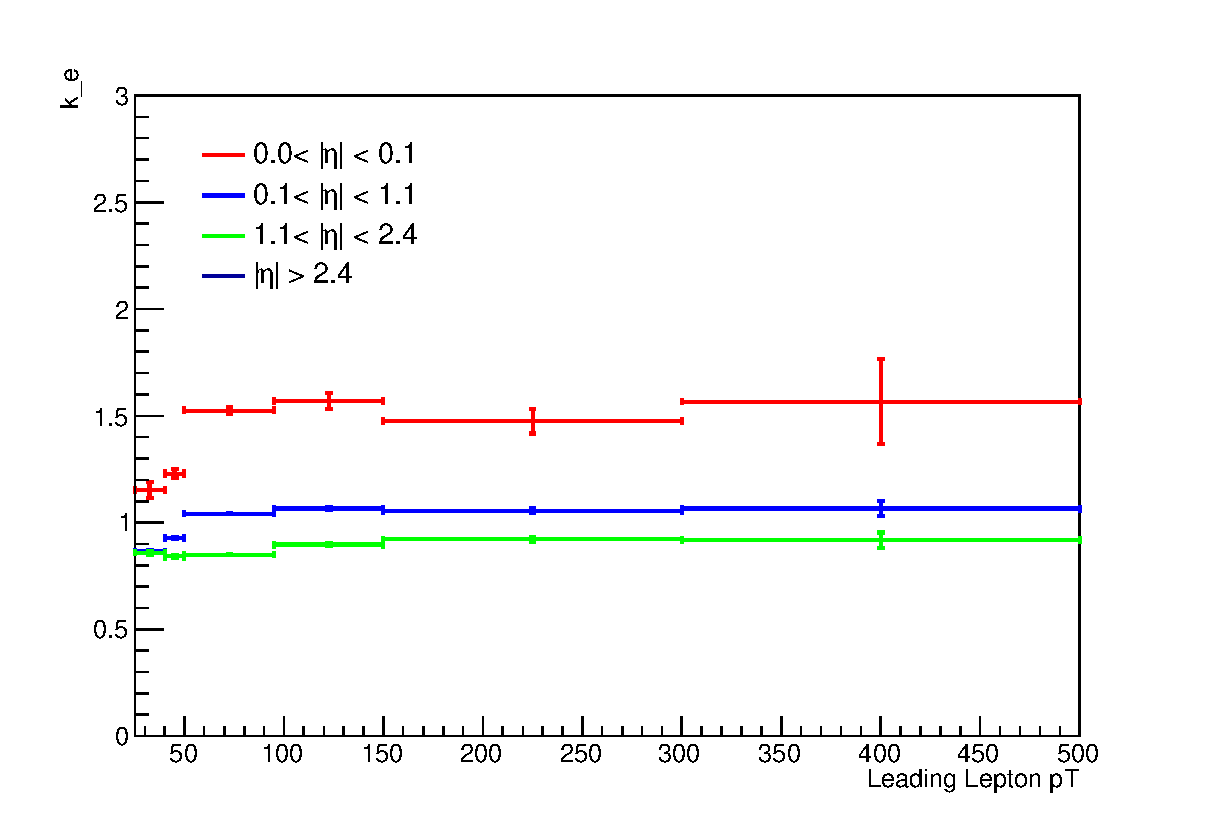
\includegraphics[width=.85\linewidth]{figures/fs/data_efficiencies_2j_Z_lep0.eps}
\caption{Comparison of data and \ac{MC} in a selection like SRZ, without the \met cut.}
\label{fig:fs_mc_met}
\end{figure}
\end{centering}

This method is extremely effective as a crosscheck because it uses a completely independent dataset from the flavor symmetry method, and the two methods have very little overlap in dependence on \ac{MC}. They produce consistent results in both SRZ and VRS, as shown in \autoref{tab:fs_comparison}.


\begin{table}[h]
\centering

\begin{tabular}{ccc}
\noalign{\smallskip}\hline\noalign{\smallskip}
Region  & Flavour-symmetry  & Sideband fit  \\
\noalign{\smallskip}\hline\noalign{\smallskip}
SRZ & $33 \pm 4$   &  $29 \pm 7$  \\ [+0.05cm]
VR-S & $99\pm8$        &  $92 \pm 25$  \\ [+0.05cm]
\noalign{\smallskip}\hline
\end{tabular}
\caption{ Comparison of \ac{FS} background predictions from the nominal method, the flavor symmetry method, and the cross-check, the sideband fit method. Uncertainties include statistical and systematic uncertainties in both cases. }
\label{tab:fs_comparison}
\end{table}

\section{\dyjets Background}
\label{sec:bg-z}

\section{Fakes}
\label{sec:bg-fake}

The fakes background is mostly due to semileptonic \ttbar and $W$+jets processes, which both have only one lepton in their final states. However, they can be reconstructed with two leptons due to an additional faked lepton or real non-prompt lepton. As such, it includes both events that have been properly reconstructed and many that are included in the \ac{SR} due to imperfect reconstruction. As with the \dyjets background, it is very difficult to model with \ac{MC} because the flaws in reconstruction are typically less well described by the models used in \ac{MC} production than the successes. Nonetheless, a rough estimate can be made of this background by using \ac{MC}, which indicates that the number of fake events in SRZ is consistent with zero. 

Despite the small predicted contribution, a data-driven method called the ``matrix method'' is employed to estimate these fake events. 


\section{Dibosons}
\label{sec:bg-diboson}

\section{Other Rare Processes}
\label{sec:bg-other}
